
\documentclass[a4paper,12pt]{report}
% arara: pdflatex: { draft: true }
% arara: makeglossaries
% arara: pdflatex: { synctex: true }
% arara: pdflatex: { synctex: true }
% add makeIndex:makeIndex  makeindex %.nlo -s nomencl.ist -o %.nls to commands when running in
\usepackage[square,sort,comma,numbers]{natbib}
\renewcommand{\bibname}{References}
\usepackage[a4paper,bindingoffset=0.2in,%
left=1in,right=1in,top=1in,bottom=1in,%
footskip=.25in]{geometry}
\bibliographystyle{unsrtnat}

\setcitestyle{authoryear,open={(},close={)}}
\usepackage[utf8]{inputenc}
\usepackage{epsfig}
\usepackage{latexsym}
\usepackage[hidelinks]{hyperref}
\usepackage{graphicx}
\usepackage{subcaption}
\usepackage{amssymb}

\usepackage{tikz}
\usetikzlibrary{shapes,arrows,positioning,chains}


\usepackage[font=scriptsize,labelfont=bf,format=plain,justification=raggedright, singlelinecheck=false]{caption}
\captionsetup[figure, table]{font=scriptsize,labelfont=bf,format=plain,justification=raggedright, singlelinecheck=false}

\usepackage{titlesec}
\titleformat{\chapter}[display]{\bfseries\centering}{\huge Chapter \thechapter}{1em}{\Huge}
%Load nomenclature and glossary files
\usepackage[nottoc]{tocbibind}
\usepackage[intoc]{nomencl}
  \renewcommand{\nomlabel}[1]{#1 \dotfill}

\makenomenclature
\renewcommand{\nomname}{List of Abbreviations}
\usepackage{mathtools}
\usepackage{pdfpages}

\usepackage[page,toc,titletoc,title]{appendix}
%\usepackage{refcheck}

\usepackage{datetime}

\newdateformat{monthyeardate}{%
    \monthname[\THEMONTH], \THEYEAR}

\DeclareGraphicsExtensions{.pdf,.png,.jpg}
\captionsetup{justification=centering,margin=2cm}


\begin{document}


    \title{Develop New Transformer Architecture For \\ Question and Answering}

    \author{Nirbhay P. Tandon\\ Master's of Science in Data Science\\Liverpool John Moore's University}

    \date{\vfill \monthyeardate\today}
    \maketitle


    \cleardoublepage% \clearpage
    \pagenumbering{roman}
    \tableofcontents
    \newpage
    \listoffigures
    \listoftables
    %Nomenclature

\nomenclature{RNNs}{Recurrent Neural Networks}
\nomenclature{LSTMs}{Long Short-Term Memory Architectures}
\nomenclature{NLP}{Natural Language Processing}
\nomenclature{NLU}{Natural Language Understanding}
\nomenclature{RACE}{ReAding Comprehension Dataset From Examinations}
\nomenclature{MCTest}{Machine Comprehension of Text}
\nomenclature{QASENT}{A challenge dataset for open-domain question answering}
\nomenclature{BPPTs}{Back-Propagation Through Time}
\nomenclature{SQuAD}{Stanford Question Answering Dataset}
\nomenclature{CEC}{Constant Error Carousel}
\nomenclature{BERT}{Bidirectional Encoder Representations from Transformers}
\nomenclature{RoBERTa}{Robustly Optimized BERT}
\nomenclature{ALBERT}{A LITE BERT}
\nomenclature{DistilBERT}{Distilled Version of BERT}
\nomenclature{QnA}{Question and Answering}
\nomenclature{BiLSTM}{Bidirectional LSTM}
\nomenclature{SuBiLSTM}{Suffix Bidirectional LSTM}
\nomenclature{CNNs}{Convolutional Neural Networks}
\nomenclature{EM}{Exact Match}
\nomenclature{Ans-Ptr}{Answer-Pointer layer}
\nomenclature{GloVe}{Global Vectors for Word Representation}
\nomenclature{BLEU}{Bilingual Evaluation Understudy}
\nomenclature{WMT}{Workshop on Statistical Machine Translation}
\nomenclature{GPUs}{Graphical Processing Units}
\nomenclature{FFN}{Feed Forward Network(s)}
\nomenclature{MLM}{Masked Language Model}
    \printnomenclature[1in]
	\begin{abstract}
		Attention-based Transformer architectures have become the norm of current Natural Language Processing applications. Google began this trend back in 2017 with their paper \textit{Attention Is All You Need}, by introducing the Transformer architecture that works solely on attention mechanisms. The purpose of our work will be to create a new kind of Transformer architecture. Compare and contrast its performance against other architectures such as BERT, DistilBERT, ALBERT etc. using the SQuAD 2.0 Dataset. Through our research, we aim to produce a new architecture that has a better performance than existing models specifically for Question Answering based applications.
	\end{abstract}
    \cleardoublepage% \clearpage
    \pagenumbering{arabic}
    \chapter{Introduction}\label{c1introduction}

    One of the most philosophical questions that anyone can encounter is \textit{``Can an answer exist without a question?"}. While that question exists to be solved by philosophers and thinkers, we shall aim to address the \textit{answer} that can be provided to a question in terms of the context that has been asked. While the field of Natural Language Processing(NLP) is vast and many unexplored areas exist, in this thesis the focus is entirely on developing a novel architecture that provides \textit{highly contextual and relevant answers} to the questions asked of it.

    The earliest examples of Question-Answering(QA) systems can be traced back to 1961, in the form of BASEBALL,\citep{green1961baseball}, a system developed by Bert F. Green and team to answer basic questions posed using punch cards in ordinary English language about stored data on baseball games. The team implemented a dictionary structure to allow for answers to be looked up and printed. For example, the system could answer very direct questions such as: ``Where did each team play on July 7?".
    A highly impressive feat for the early days of neural networks in the 1960s, the work done by Green paved the way for systems like LUNAR,\citep{lunar}, answered geological questions for the rocks brought back from the Apollo moon missions. LUNAR, which was first presented in 1971, had an astounding 90\% accuracy rate for questions that were asked by people who didn't know how the system worked!
    Question-Answering based systems have gained a lot of popularity, especially in the form of ``chatbots''. These systems depend highly on contextual understanding of the input, the training corpus and the question asked. They use this knowledge to output an answer that can help the user with whatever their query is. Recurrent neural networks and architectures based on them, have been able to provide great advancements in the field of Question-answering and chatbots in general. However, there is a behaviour of over-fitting and a lack of contextual understanding of the question. This, coupled with long training times and extremely complex mathematical model designs, have often kept the field of Natural Language Processing slightly obscured from the masses.


    The task of Question-Answering is a machine comprehension problem. If we dig deeper, we can classify it even as a sequential problem. One might wonder how it is a sequential problem? The answer to that is simple, traditionally QA systems work by ``sequentially reading" the input and
    In a more mathematical context, we can say that the problem we face is of \textit{answer selection} and not \textit{answer provision}. Through numerous studies that have been done, some of which we shall look into detail in chapter \ref{c2litrev}, we see that the problem is not how to provide an answer to a question, it is if the answer provided is the correct one or not in the \textit{context} in which the question has been posed.

    Through the work done in this research, the author aims at creating a sustainable, fast, easy to understand Transformer architecture for Question Answering. An advancement on the work done by the team at Google \citep{atayl}. To be able to do so, let us first understand what a \textit{Transformer} is.
    A Transformer is a form of transduction model that relies solely on self-attention to figure out how to represent its inputs and outputs. It does so without the use of any sequence aligned recurrent neural networks(RNNs) or convolutions.


        \section{Background Of The Study}\label{c1background}
        	In this section, we shall highlight what has led us this far and some of the interesting challenges that it poses. In \ref{back}, we briefly look at the history of Natural Language Processing and how some of the challenges were addressed. In \ref{rr}, we look at the latest research that has gone into creating the Transformer architecture, identify some of the common patterns and use that information to strategise our model in later sections.

            The area of Natural language Processing has taken significant leaps in the last two decades. Work done towards improving the ability of machine learning models to first recognize words, then sentences, followed by contextual understanding has led to several interesting and novel approaches in the field. From early on neural networks to creating Long Short-Term Memory architectures \citep{lstmoriginal} by Sepp Hochreiter and Jurgen Schmidhuber in the mid-'90s that resolved the vanishing gradient problem of classical neural networks, we have come a long way.

           The latest advancements in this field come from Google's research lab in the form of \textit{Transformers}. We look into this in a bit more detail later. However, no model can be successful without a good dataset to train on. This is where the SQuAD 2.0 dataset \citep{dataset} comes in. This dataset is what forces the machine learning models to do contextual understanding. One might even say that it forces the models to ``think'' for themselves before answering a task.

           Let us now look at some of the key research that has been done in this regard.


        \section{Aims And Objectives}\label{12}
        	The main aim of this research is to propose an improvement to the transformer architecture that can perform better at Q\&A using the SQuAD 2.0 dataset.
        We shall:
        \begin{enumerate}
        	\item Implement the existing models that are available via libraries such as HuggingFace \citep{hfTransformers} and PyTorch  on the dataset
        	\item Obtain F1, Exact Match(EM), etc. scores for existing models and treat them as our benchmark scores
        	\item Identify drawbacks of the current architectures
        	\item Design our architecture and evaluate its performance
        	\item Fine-tune the architecture, re-evaluate and report improvements yes yes yes
        	\item Compare the results of our Transformer model with the benchmark scores.
        \end{enumerate}

        \section{Scope Of The Study}\label{13}

        This research work is entirely focused on the area of Question-Answering based networks. This focus helps in significantly narrowing down the scope and critically assessing the problem that needs to be solved. The practical applications of the field of QA are endless. From chatbots to QA systems on domain-specific knowledge or conversational applications for voice assistants, a light, robust, highly accurate Transformer based architecture can help ease the daily lives of millions of users.
        \section{Significance Of The Study}\label{14}

        The current state of the art systems, some of which have been highlighted in section \ref{c1background}, suffer from various drawbacks and even the best models have only been able to achieve an EM score of 90.871 with an F1 score of 93.183 on the SQuAD 2.0 leaderboard \citep{squad}.
        \section{Structure Of The Study}\label{15}
           We have divided this report into 3 main chapters. Each chapter is broken down into sections and subsections to localize the reference and use it further in the global context of this research. In chapter \ref{c1introduction}, an introduction to the concept of Question-Answering, a brief look at the problem, the motivation, the scope of this research and its significance have been provided. Chapter \ref{c2litrev}, looks in detail at the background studies that have been briefly mentioned in section \ref{c1background}. In this chapter critical analysis is conducted how some of the work that has been selected is relevant to what this research aims to highlight, it helps us understand the merits and shortcomings of current state of the art approaches. Finally, Chapter \ref{c3researchmeth}, details the research methodology used by the author. Chapter \ref{c3researchmeth} helps the reader understand various nuances of the dataset, evaluation metrics, pre-processing techniques, benchmarks from existing systems etc.
           Appendix \ref{cgc} is where the reader can refer to the Gantt chart for the thesis work done and the updates to various stages.

    \chapter{Literature Review}\label{c2litrev}

    To be able to effectively deliver on the aims and objectives we have defined in Section \ref{12}, we must first critically analyse the work that has been done in the field of NLP and, in particular, the field of Question-Answering based networks. In this section, we will critically analyse a few key model architectures and how we reached Transformers, which form the base of our proposed architecture.

\citep{fastQA}

        \section{Long Short-Term Memory}\label{22}

            In 1997 \citep{lstmoriginal} introduced to the world a gradient descent based model in the form of Long Short-Term Memory. They set out to solve the problem of the vanishing gradient which was often seen in "Back-Propagation Through Time"(BPPTs) based neural networks. Extensive studies done on this, some by Hochreiter himself, showed that the problem of vanishing gradients is a real one. It was also seen that in case of BPTTs, the error back-flow mechanisms would either blow up or also suffer from vanishing gradients leading to either oscillating weights or learning to bridge long time gaps would not work. To remediate this, the authors introduced the concept of a \textit{constant} error flow through the internal states of special units.

            Their paper, Long Short-Term Memory, \citep{lstmoriginal}, highlights that the work previously done using various gradient-descent variants, time-delays, time constants, use of higher order units to influence connections when the network receives conflicting error signals, Kalman filters, Second order nets etc. still suffer from some of the same problems that we have earlier. In the case of Ring's approach \citep{lstmRing}, the network can be really fast but also suffers from memory constraints and lack of generalization. This happens because to bridge $ n $ time lags, the model adds $ n $ additional units.

            It is essential for us to understand how LSTMs function as it forms the basis of Transformers to exist. Hochreiter and Scmidhuber designed a \textit{memory cell} that  allows for a constant error flow. This is achieved by introducing \textit{constant error carousel}(CEC), a multiplicative input gate unit and a multiplicative output gate unit. These \textit{multiplicative} units help shield the contents of the memory cell from irrelevant inputs. The CEC, input and output gates together form the \textit{memory cell}, as seen in Fig. \ref{lstmCEC}.
           	\begin{figure}[h!]
      				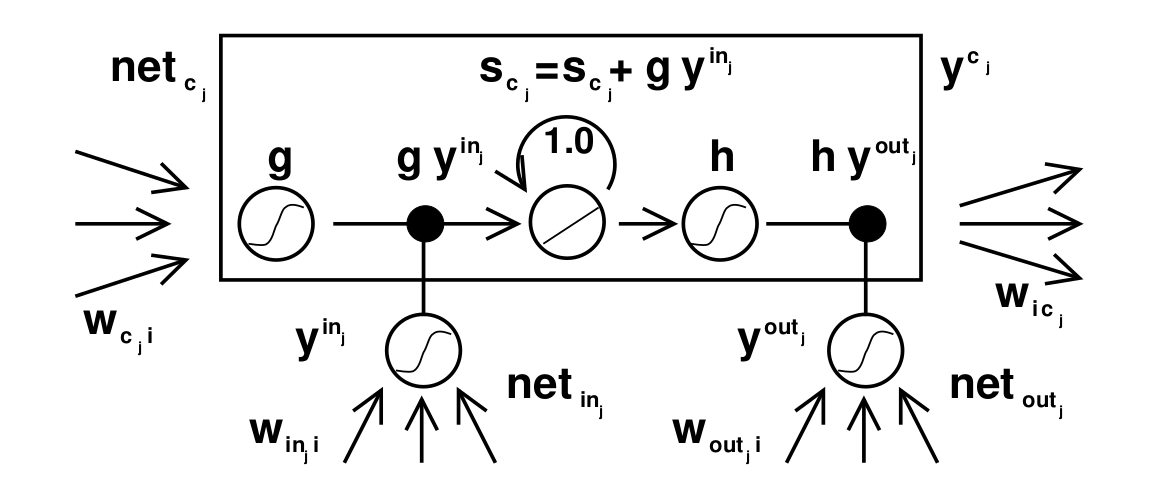
\includegraphics[scale=0.35]{../images/lstm-memorycell.png}
      				\caption{LSTM Memory cell with a Constant Error Carousel having fixed weight 1.0, \citep{lstmoriginal}}\label{lstmCEC}
             \end{figure}
            The central feature for LSTM's memory cell is the CEC. The self-recurrent connection, where weight is 1.0, is what helps create a time-delayed feedback loop by 1.

            The CEC uses gate units to circumvent the issue with conflicting weights in the input and output layers. The input layer has control over when to use and when to override the information in the CEC but has no control over the error signals that are in the memory cell. The output gate, however, uses a feedback mechanism to assess when to superimpose different error signals. It also falls on the output gate to \textit{learn} which errors to trap in the CEC by appropriately scaling them. The gates have to learn when to release and trap errors therefore controlling the access to the CEC, helping maintain constant error flow. To mathematically understand the memory cell from fig. \ref{lstmCEC}, Schmidhuber and Hochreiter proposed the following set of equations \ref{eq1} - \ref{eq3}. More details on this can be found by referring to the appendix section A.1 in \citep{lstmoriginal}.
            \begin{equation}\label{eq1}
                y^{{out }_{j}}(t)=f_{ {out }_{j}}\left( { net }_{ {out }_{j}}(t)\right) ; y^{i n_{j}}(t)=f_{i n_{j}}\left( { net }_{i n_{j}}(t)\right)
            \end{equation}
	        where
            \begin{equation}\label{eq2}
                net_{out_{j}}(t)=\sum_{u} w_{out_{j} u} y^{u}(t-1)
            \end{equation}
            and
            \begin{equation}\label{eq3}
                            net_{in_{j}}(t)=\sum_{u} w_{in_{j} u} y^{u}(t-1)
            \end{equation}
            A generalised form of this equation can be represented as:
            \begin{equation}\label{eq4}
                            net_{c_{j}}(t)=\sum_{u} w_{c_{j} u} y^{u}(t-1)
            \end{equation}
            At time $ t $, $ c_{j} $'s output $ y^{c_{j}}(t) $ is computed as:
            \begin{equation}\label{eq5}
                y^{c_{j}}(t) = y^{out_{j}}(t)h(s_{c_{j}}(t)),
            \end{equation}
            where the ``internal state'' $ s_{c_j}(t) $ is:
            \begin{equation}\label{eq6}
                s_{c_{j}}(0)=0, s_{c_{j}}(t)=s_{c_{j}}(t-1)+y^{i n_{j}}(t) g\left( { net }_{c_{j}}(t)\right) \textrm{for } t>0
            \end{equation}
            Where $ u $ may stand for input, output or gate units, memory cells or even conventional hidden units, if they are being used.

            In fig. \ref{lstmNetwork}, we see the internal workings of how an LSTM network could look like.
            \begin{figure}[!h]
	           \centering
               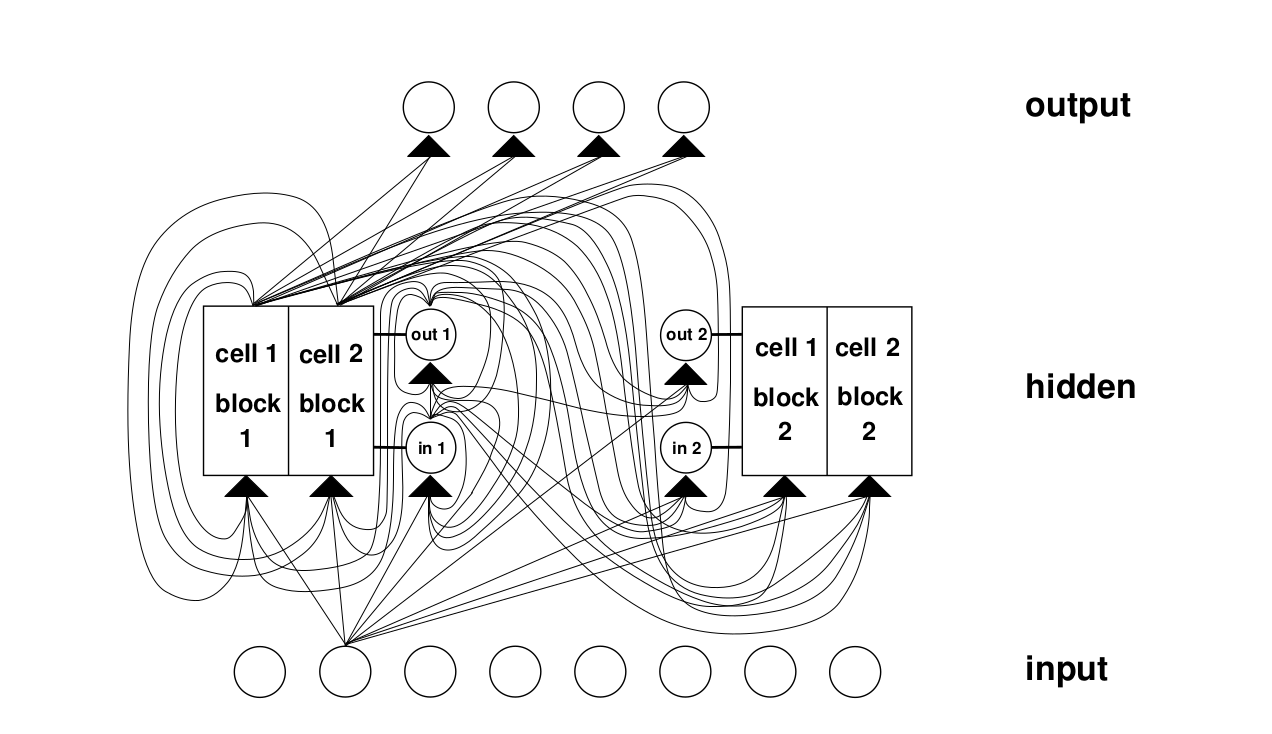
\includegraphics[scale=0.35]{../images/lstm-network.png}
      		   \caption{LSTM network with 8 input cells, 4 output cells and 2 memory cells of block size 2. Here $ in1 \text{and} out1 $ represent the input and output gates and $ cell/block1 $ is the first memory cell. The internal architecture of $ cell/block1 $ is similar to fig. \ref{lstmCEC}. \citep{lstmoriginal}}\label{lstmNetwork}
            \end{figure}

            A series of experiments were performed to prove that LSTMs are indeed ``state-of-the-art" and provide an improvement over then existing RNN based architectures.
            Experiments around temporal order, which is defined as a series of events that happen in a particular order, that were previously unsolved by RNNs, were successfully solved by LSTMs. This was possible because of how LSTMs address time lags vs. how RNNs suffer from vanishing gradients. Details of the analysis and experiments conducted are available in section 5 of the paper ``Long Short-Term Memory" by \citep{lstmoriginal}, with experimental summaries in tables 10 and 11 of the same. Being able to solve for temporal order based problems allowed LSTMs to be capable of solving various real world problems that we will discuss subsequently.
            Temporal orders are key in contextual understanding for NLP based tasks and especially in the case of QA based networks. Let us now look at some advantages and limitations of LSTMs, before moving on to understand how they have been applied in the field of QA.


            \subsubsection{Advantages of LSTMs}
                \begin{itemize}
                    \item LSTMs deal with long time lags by bridging the gaps using constant error flow in the memory cells.
                    \item LSTMs respond well to generalization problems, even if the input sequences are widely separated.
                    \item They work well with a variety of braod range hyper-parameters and don't usually require tuning.
                    \item Their time and weight update complexity is the same as BPTT, ie. $ O(1) $. The advantage for LSTMs however, is that it is local in both space and time.
                \end{itemize}

            \subsubsection{Limitations of LSTMs}
                \begin{itemize}
                    \item LSTMs use memory cells which require an additional input and output unit. This \textit{hidden unit} is replaced by 3 units in an LSTM architecture, compared to 9 in an RNN. A fully connected LSTM will have $ 3^{2} $ connections however.
                    \item LSTMs dont work well when they get the entire input in one go. The architecture is unable to generalize well by random weight guessing in this case.
                    \item They do not have the ability to ``natively" count discrete time steps which might be useful in some applications. This isn't a big issue for the case of QA based problems.
                \end{itemize}

             \subsection{BiLSTMs}\label{c2bilstm}
                  \begin{figure}[!h]
     	           \centering
                    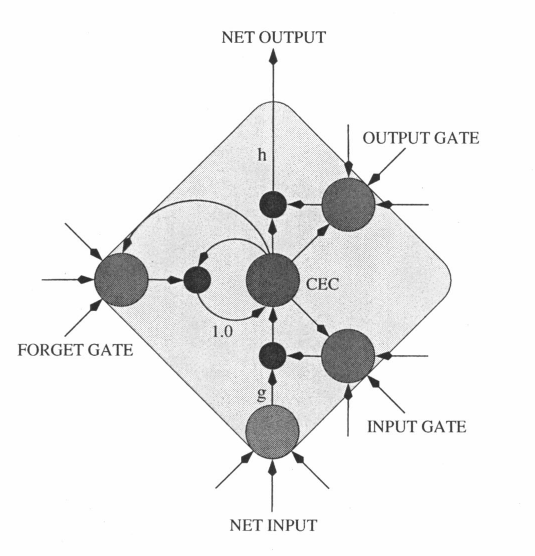
\includegraphics[scale=0.35]{../images/lstm-biLstm.png}
           		   \caption{A memory cell for a biLSTM highlighting a \textit{forget gate}. This forget gate helps in scaling the internal state of a memory cell, for example by resetting the state to 0. We can see that it is different to fig. \ref{lstmCEC}, with the implementation of a connection to the forget gate, while still having an internal weight of 1. \citep{lstmBiLSTM}}\label{lstmBilstm}
                 \end{figure}
            While LSTMs have found various applications across the field of machine and deep learning, QA seems to be one where being able to achieve consistent results of accuracy as well as having an exact match seems to elusive.
            Research carried out at IBM by Tan, Santos and co. looked at approaching this problem by using something called Bidirectional LSTMs or BiLSTM, \citep{lstmBiLSTM}. Introduced by Graves and Schmidhuber in their paper \textit{Framewise Phoneme Classification with Bidirectional LSTM Networks}, the biLSTM implements a \textit{forget gate} as seen in fig. \ref{lstmBilstm}. An advantage of biLSTMs over traditional LSTMs is that you feed the data twice, once from the beginning to the end and then from the end to the beginning. This helps the model contextualize and adjust weights better, therefore creating a more robust model that learns and performs better overall when compared to traditional LSTMs and RNNs.
             \begin{table}[h!]
              \centering
                \begin{tabular}{|c|c|c|c|}
                    \hline
                     & Questions & Answers & Question Word Count \\
                    \hline
                    Train & 12887 & 18540 & 92095 \\
                    \hline
                    Dev & 1000 & 1454& 7158 \\
                    \hline
                    Test1 & 1800 & 2616 & 12893 \\
                    \hline
                    Test2 & 1800 & 2593 & 12905 \\
                    \hline
                \end{tabular}
                \caption{InsuranceQA Corpus Details: Some questions can have multiple answers, therefore the number of answers is greater than the number of questions \citep{lstmInsuranceQA}.}\label{lstmInsuranceQATable}
            \end{table}

            BiLSTMs were introduced as an approach towards phoneme classification for speech recognition applications, however, in their paper ``LSTM-BASED DEEP LEARNING MODELS FOR NON -FACTOID ANSWER SELECTION", \citep{lstmhaighextractive} have shown that extending the biLSTM model 2 different approaches for QA has its advantages. One approach, using a more composite method of using CNNs for representing questions as well as answers. The other, by implementing an \textit{attention mechanism} that helps in generating an answer representation according to the question context.
            Their framework is based on developing a biLSTM model for both questions and answers, applying a connective pooling layer and using a cosine similarity metric to calculate the degree of matching answers. They utilized the InsuranceQA\citep{lstmInsuranceQA} dataset that was created in 2015 and tested primarily on CNN based networks, details of the dataset can be found in table \ref{lstmInsuranceQATable}.

            \begin{figure}
            	\centering
            	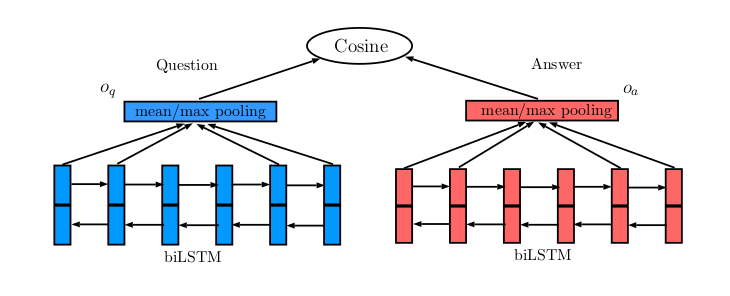
\includegraphics[scale=0.4]{../images/lstm-bilstmhaig.png}
            	\caption{Basic QA-LSTM model depicting biLSTM implementation \citep{lstmhaighextractive}}\label{lstmhaig}
            \end{figure}

            Pooling layers are known to suffer from an incapability to retain local linguistic information. To combat this the team proposed an additional CNN layer on top of the biLSTM layer. Additionally, they added a simple and efficient attention model to help their biLSTM model better distinguish between candidate answers according to the question context. This study is significant in the field of both deep learning based models and for the field of Question-Answering because it requires little or no feature engineering to achieve significant results. We will also see later in section \ref{23}, how biLSTMs are implemented with Transformers to produce an even better model.
            In their work \citep{lstmhaighextractive} have shown that biLSTMs are capable of capitalizing long-range sequential context information. This is important as it is often seen that the answer is not directly semantically related to the question but more contextually related. Long-range exploitations help the model understand the question more holistically, therefore helping produce a more relevant answer.


		   \begin{figure}
				\centering
				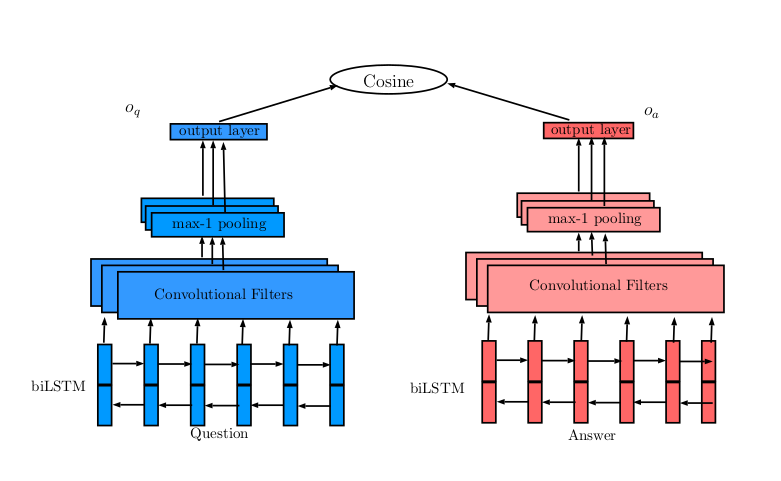
\includegraphics[scale=0.35]{../images/lstm-bilstmhaigcnn.png}
				\caption{QA-LSTM with CNN layer \citep{lstmhaighextractive}}\label{lstmhaigcnn}
			\end{figure}

             BiLSTMs have an advantage over traditional LSTMs in that they utilize both previous and future contextual information by processing the input in both directions, forward and backward. This leads to the generation of two independent sequences of output vectors form LSTMs. The final output is a concatenation  of the outputs from both directions ie. $h_t= \overrightarrow{h_t} || \overleftarrow{h_t} $.
             The \textbf{QA-LSTM} model  proposed by \citep{lstmhaighextractive} can be seen in fig. \ref{lstmhaig}. We can see that it generates a distributed representation for both questions(blue) and answers(red) before moving on to perform pooling and cosine similarity operations.
            In fig. \ref{lstmhaigcnn}, it can be seen that the CNN layer has been implemented after the biLSTM layers and before the pooling layers. The pooling layers have been modified to be max-$ k $ pooling layers, similar to standard CNNs.


            The implementation of this convolution layer forces localized interactions between the inputs within a filter size of $ m $. For each window of size $ m $ in biLSTM output vectors ie.
            \begin{equation}
            \textbf{H}_{m}(t)=[\textbf{h}(t), \textbf{h(t+1)},...,\textbf{h}(t+m-1)]
            \end{equation}
            where $ t $ is a time step and the convolution filter will generate one value as follows
            \begin{equation}
                o_{F}(t) = tanh \bigg[\bigg(\sum_{i=0}^{m-1}\textbf{h}(t+i)^{T}\textbf{F}(i)\bigg)+b\bigg]
            \end{equation}

            Using $ k $-MaxPooling, the authors emphasized that a maximum of $ k $ values will be kept  for one filter, thereby indicating the highest degree that a filter matches the input sequence. To end this approach, there are $ N $ parallel filters, with different parameter initialization which provide the CNN layer with $ N $-dimension output vectors. This produces two output vectors of dimension $ kN $ for each question and answer.  Their experiments intuitively took $k=1$ as anything greater showed no improvements and it helped emphasize aspects of the answer such that this CNN based hybrid biLSTM could differentiate ground truths and incorrect answers efficiently.

            The second approach adopted in this paper is actually inspired by another paper \citep{bilstmHerman} where attention based deep LSTM networks were used to enhance the capabilities of reading comprehension in LSTM based models. Here, in \citep{lstmhaighextractive}, a modification has been introduced in the form of attention-based connections along with biLSTM layers as depicted in fig. \ref{lstmhaigattention}.
            \begin{figure}
                \centering
                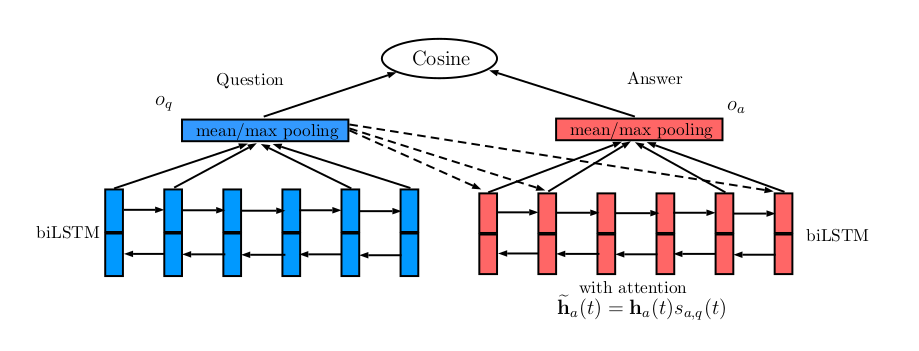
\includegraphics[scale=0.35]{../images/lstm-bilstmhaighattention.png}
                \caption{QA-LSTM with Attention layer \citep{lstmhaighextractive}}\label{lstmhaigattention}
            \end{figure}

            Before conducting a mean/average pooling operation on the output from every biLSTM, the output vectors are multiplied by a softmax weight that is determined by the question embeddings from the biLSTM.
            It was shown that given an output vector from a biLSTM for an answer at time $ t, \textbf{h}_{a}(t)$ and the question embedding, $ o_q $, the updated vector $  \tilde{\textbf{h}_{a}}(t)$ for each answer token
            can be given as:
            \begin{equation}\label{bilstmAttentioneq}
                \textbf{m}_{a,q}(t) = tanh(\textbf{W}_{am}\textbf{h}_{a}(t) + \textbf{W}_{qm}o_{q})
            \end{equation}
            \begin{equation}\label{bilstmattentioneq2}
                s_{a,q}(t) \propto exp(\textbf{w}^{T}_{ms}\textbf{m}_{a,q}(t))
            \end{equation}
            \begin{equation}\label{bilstmattentioneq3}
               \tilde{\textbf{h}_{a}} = \textbf{h}_{a}(t)s_{a,q}(t)
            \end{equation}
            where  $ \textbf{W}_{am}, \textbf{W}_{qm} $ and $ \textbf{w}_ms $ are attention parameters. Attention parameters show somewhat similar behaviour to tf-idf  where some words get more attention or weights associated to them. The main difference being that the attention mechanism adjusts its weights according to question information.

            Critically, this attention based approach from \citep{lstmhaighextractive} emphasizes on attention-driven representations and uses that to calculate the distances between questions and their respective answers. A combination approach with CNNs and attention based connections helps in localizing various internal connections, correctly scaling the errors and reducing unnecessary noise. From eq. \ref{bilstmAttentioneq}-\ref{bilstmattentioneq3}, \citep{lstmhaighextractive} we can mathematically prove how the average distances are computed.
            Experiments conducted on the InsuranceQA dataset showed that the \textit{QA-LSTM/CNN with Attention} model can outperform the taken baseline models, which were based purely on QAs using CNNs.
            \begin{table}
                \begin{tabular}{|l|llll|}
                    \hline & Model & Validation & Test1 & Test2 \\
                    \hline A & QA-LSTM basic-model(head/tail) & $54.0$ & $53.1$ & $51.2$ \\
                    B & QA-LSTM basic-model(avg pooling) & $58.5$ & $58.2$ & $54.0$ \\
                    C & QA-LSTM basic-model(max pooling) & $64.3$ & $63.1$ & $58.0$ \\
                    \hline D & QA-LSTM/CNN(fcount=1000) & $65.5$ & $65.9$ & $62.3$ \\
                    E & QA-LSTM/CNN(fcount=2000) & $64.8$ & $66.8$ & $62.6$ \\
                    F & QA-LSTM/CNN(fcount=4000) & $66.2$ & $64.6$ & $62.2$ \\
                    \hline G & QA-LSTM with attention (max pooling) & $66.5$ & $63.7$ & $60.3$ \\
                    H & QA-LSTM with attention (avg pooling) & $\mathbf{6 8 . 4}$ & $\mathbf{6 8 . 1}$ & $62.2$ \\
                    I & QA-LSTM/CNN (fcount=4000) with attention & $67.2$ & $65.7$ & $\mathbf{6 3 . 3}$ \\
                    \hline
                \end{tabular}
                \caption{Experimental results from \citep{lstmhaighextractive}, highlighting how QA-LSTM with attention outperforms its various modifications}\label{lstmhaigexperiementresults}
            \end{table}

			  An improvement to this approach was done in 2018 by \citep{lstmSubilstm} who proposed \textit{Suffix Bidirectional LSTM} or \textit{SuBiLSTM} adding prefixes and suffixes to the inputs over both directions.  There are a few obvious differences between the biLSTM and SuBiLSTM like the doubling of parameters, increased time complexity which happens over quadratic time for worst case scenarios compared to linear in biLSTMs.
			  The author of this paper has shown that despite higher time complexity, there are significant gains in accuracy in text encoding and classification in their experiments, of particular note is the Paraphrase Detection experiment which uses GloVe embeddings and shows an 88.2\% score in the test set, which is marginally higher than other models implemented.
			  The work presented in this thesis will also implement paraphrase detection and GloVe embeddings to potentially improve model performance and answer detection.

			  \subsection{LSTM And Question Answering}\label{c2lstmqa}
             In 2016, The SQuAD dataset \citep{dataset1} was released, that generated quite a buzz in the field of QA based NLP tasks due to its nature of being extremely versatile and crowdsourced. We will take  a deeper look at it in section \ref{24}, where we discuss the various datasets in detail.

             Using the SQuAD dataset \citep{lstmhu2016question} developed a match-LSTM \citep{lstmMatch} based model that they showed performed significantly better on the dataset than the work done by \citep{dataset1}. Their work shows that using a match-LSTM approach combined with a Pointer Net model \citep{lstmPointer}, that aids token predictions using only input sequences rather than using any form of large fixed vocabulary, therefore allowing for generation of answers with multiple tokens.

             The approach by \citep{lstmhu2016question} was tw-fold. The first approach implemented as a sequence model and the second as a boundary model, which was further extended with a search function.

             The match-LSTM model architecture consists of:
             \begin{itemize}
             	\item \textbf{LSTM Preprocessing Layer}: As we can see from \ref{lstmMatch}, there are 2 LSTM preporcessing layers. This layer is used to integrate contextual information directly into the representation of how each token in the passage and question is represented. This is based directly on the simple LSTM \citep{lstmoriginal} and not the BiLSTM.
             	\item \textbf{Match-LSTM Layer}: Here, the model treats the question as a premise and the passage as hypothesis. The layer sequentially reads the passage and calculates an attention weight vector $ \vec{\alpha}_{i} \in \mathbb{R}^{Q}$ as:
             	\begin{equation}\label{eqmatchlstm}
             		\begin{aligned}
             			&\overrightarrow{\mathbf{G}}_{i}=\tanh \left(\mathbf{W}^{\mathrm{q}} \mathbf{H}^{\mathrm{q}}+\left(\mathbf{W}^{\mathrm{p}} \mathbf{h}_{i}^{\mathrm{p}}+\mathbf{W}^{\mathrm{r}} \overrightarrow{\mathbf{h}}_{i-1}^{\mathrm{r}}+\mathbf{b}^{\mathrm{p}}\right) \otimes \mathbf{e}_{Q}\right) \\
             			&\vec{\alpha}_{i}=\operatorname{softmax}\left(\mathbf{w}^{\top} \overrightarrow{\mathbf{G}}_{i}+b \otimes \mathbf{e}_{Q}\right)
             		\end{aligned}
             	\end{equation}

			where $\mathbf{W}^{\mathrm{q}}, \mathbf{W}^{\mathrm{p}}, \mathbf{W}^{\mathrm{r}} \in \mathbb{R}^{l \times l}, \mathbf{b}^{\mathrm{p}}, \mathbf{w} \in \mathbb{R}^{l}$ and $b \in \mathbb{R}$ are parameters to be learned, $\overrightarrow{\mathbf{h}}_{i-1}^{\mathrm{r}} \in \mathbb{R}^{l}$ is the hidden vector of the one-directional match-LSTM at position $i-1$, and the outer product $\left(\cdot \otimes \mathbf{e}_{Q}\right)$ produces a matrix or row vector by repeating the vector or scalar on the left for $Q$ times.
			To simply summarise, the above equation \ref{eqmatchlstm} produces  $ \vec{\alpha}_{i,j} $ that gives us the degree of matching between token $ i $ in the passage with token $ j $ in the question. This is the forward pass representation of the mathc-LSTM, the backward pass, which generates encodings for each token in the passage is given by:
			\begin{equation}\label{eqmatchlstmreverse}
				\begin{aligned}
					&\overleftarrow{\mathbf{G}}_{i}=\tanh \left(\mathbf{W}^{\mathrm{q}} \mathbf{H}^{\mathrm{q}}+\left(\mathbf{W}^{\mathrm{p}} \mathbf{h}_{i}^{\mathrm{p}}+\mathbf{W}^{\mathrm{r}} \overleftarrow{\mathbf{h}}_{i+1}^{\mathrm{r}}+\mathbf{b}^{\mathbf{p}}\right) \otimes \mathbf{e}_{Q}\right) \\
					&\overleftarrow{\alpha}_{i}=\operatorname{softmax}\left(\mathbf{w}^{\top} \overleftarrow{\mathbf{G}}_{i}+b \otimes \mathbf{e}_{Q}\right)
				\end{aligned}
			\end{equation}

		The equations above, \ref{eqmatchlstm} and \ref{eqmatchlstmreverse} are presented in \citep{lstmhu2016question}.
             	\item \textbf{Answer Pointer Layer}: This layer, the Answer-Pointer layer(Ans-Ptr), introduced by \citep{lstmPointer}. It uses the sequence $ \textbf{H}^{r} $ as input.
             \end{itemize}
         	  \begin{figure}
	         	\centering
	         	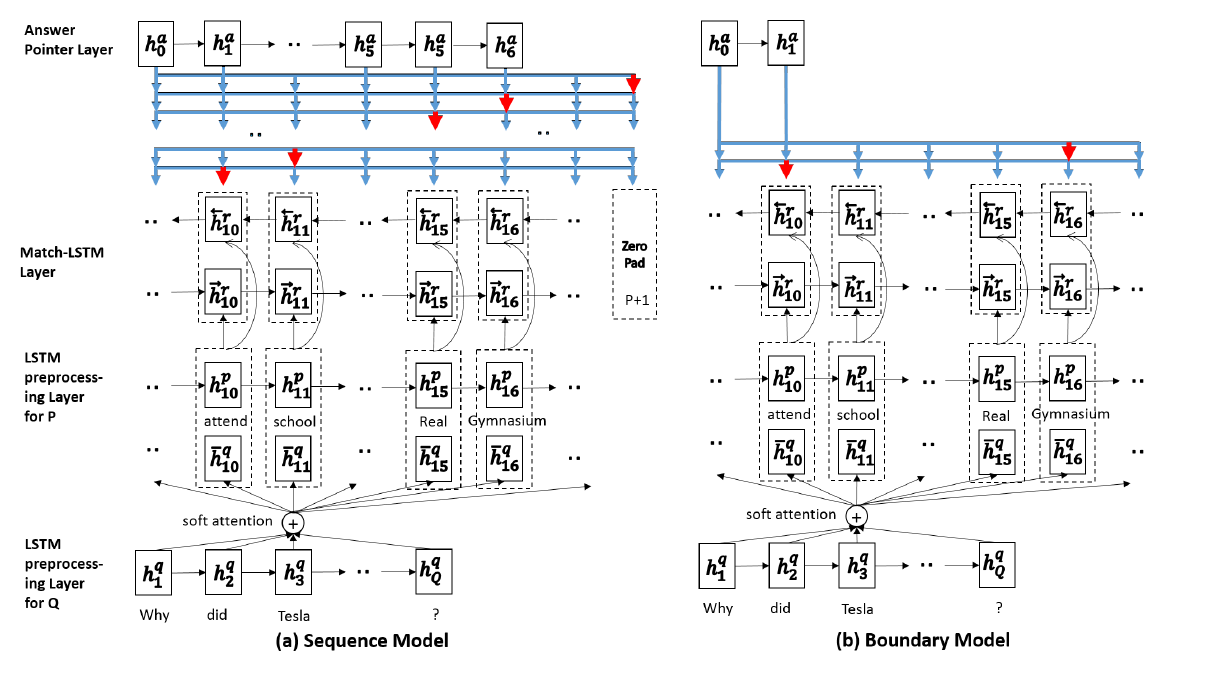
\includegraphics[scale=0.4]{../images/lstmMatch.png}
	         	\caption{Overview of the 2 approaches by \citep{lstmhu2016question}, showing the Sequence Model on the left and the Boundary Model on the right.}\label{lstmMatch}
	         \end{figure}

		It is important to highlight that the sequence model represents the answers as integers in a sequence that refer to the position of the selected token in the original passage. The Ans-Ptr layer models these sequentially as well. For the purposes of this thesis we will focus on the boundary model from the paper by \citep{lstmhu2016question}. As we can see from table \ref{tableMatchLSTM}, the results are significantly better for SQuAD 1.1 dataset. Further enhancements to this have been made and various other models have come out on top, however this paper pioneered the use of a bidirectional Ans-Ptr approach.
		\begin{table}[!htbp]
			\centering
		\resizebox{\columnwidth}{!}{
			\begin{tabular}{lcccccc}
			\hline & $l$ & $|\theta|$ & \multicolumn{2}{c}{ Exact Match } & \multicolumn{2}{c}{ F1 }\\
			& & & Dev & Test & Dev & Test \\
			\hline Random Guess & $-$ & 0 & $1.1$ & $1.3$ & $4.1$ & $4.3$ \\
			Logistic Regression & $-$ & $-$ & $40.0$ & $40.4$ & $51.0$ & $51.0$ \\
			DCR & $-$ & $-$ & $62.5$ & $62.5$ & $71.2$ & $71.0$ \\
			\hline Match-LSTM with Ans-Ptr (Sequence) & 150 & $882 \mathrm{~K}$ & $54.4$ & $-$ & $68.2$ & $-$ \\
			Match-LSTM with Ans-Ptr (Boundary) & 150 & $882 \mathrm{~K}$ & $61.1$ & $-$ & $71.2$ & $-$ \\
			Match-LSTM with Ans-Ptr (Boundary+Search) & 150 & $882 \mathrm{~K}$ & $63.0$ & $-$ & $72.7$ & $-$ \\
			Match-LSTM with Ans-Ptr (Boundary+Search) & 300 & $3.2 \mathrm{M}$ & $63.1$ & $-$ & $72.7$ & $-$ \\
			Match-LSTM with Ans-Ptr (Boundary+Search+b) & 150 & $1.1 \mathrm{M}$ & $63.4$ & $-$ & $73.0$ & $-$ \\
			Match-LSTM with Bi-Ans-Ptr (Boundary+Search+b) & 150 & $1.4 \mathrm{M}$ & $\mathbf{6 4 . 1}$ & $\mathbf{6 4 . 7}$ & $\mathbf{7 3 . 9}$ & $\mathbf{7 3 . 7}$ \\
			\hline Match-LSTM with Ans-Ptr (Boundary+Search+en) & 150 & $882 \mathrm{~K}$ & $\mathbf{6 7 . 6}$ & $\mathbf{6 7 . 9}$ & $\mathbf{7 6 . 8}$ & $\mathbf{7 7 . 0}$ \\
			\hline
		\end{tabular}
	}
		\caption{Experiment results from \citep{lstmhu2016question} that highlight various configurations implemented. The best being Match-LSTM with Ans-Ptr using a boundary, search and ensemble technique.}\label{tableMatchLSTM}
		\end{table}
		\begin{figure}[!h]
			\centering
			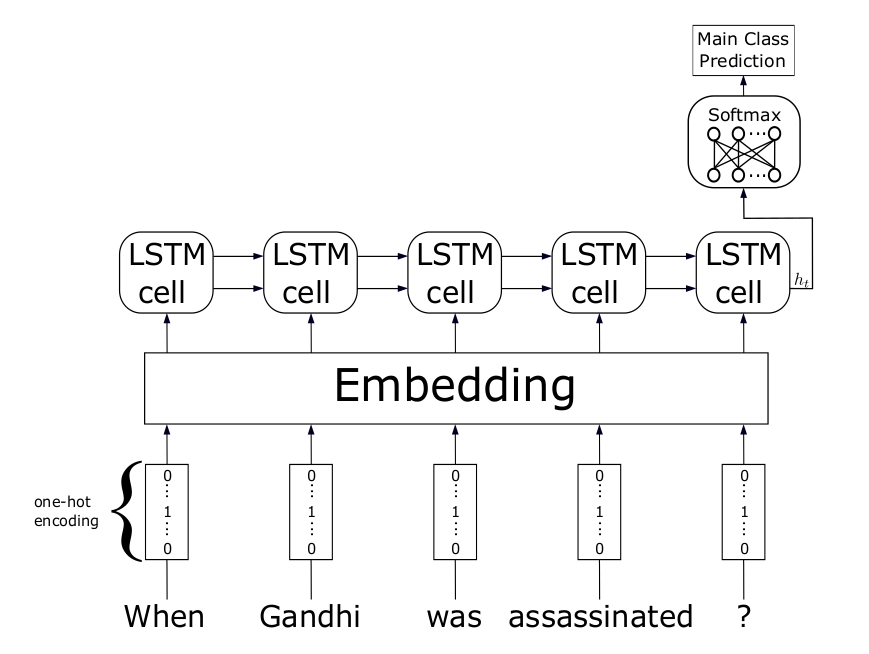
\includegraphics[scale=0.35]{../images/lstm-intent1.png}
			\caption{Basic classification model using LSTM \citep{lstmintent}}\label{lstmIntent1}
		\end{figure}
	     Our research has shown that this approach hasn't yet been applied to the SQuAD 2.0 dataset. In chapter \ref{c3researchmeth}, section \ref{c33} we will hypothesize the implementation of this approach along with the use of Transformers, which are covered in the next section.

         The final piece of research to look at in this section is by \citep{lstmintent} titled \textit{Intent Classification in Question-Answering Using LSTM Architectures}. The approach followed is similar to \citep{lstmSubilstm}, using GloVe embeddings, allowing for prefixes to be added and generating word closeness and using a supervised learning technique. In fig. \ref{lstmIntent1} it can be observed how applying one-hot encoding, followed by GloVe embedding before reaching the LSTM layer and using a Softmax activation layer at one prediction classes allows the model to generate better predictions on the TREC \citep{trec} dataset.

		In fig. \ref{lstmIntent2} we see the implementation of a padding layer at the end of each question and adding a subclass prediction strategy at the end of each prediction. This is done to gain better contextual understanding of the question. The subclass acts as a specialization class while the main class acts as a generalization class, therefore narrowing the context while maintaining global outlook.
		\begin{figure}[!h]
			\centering
			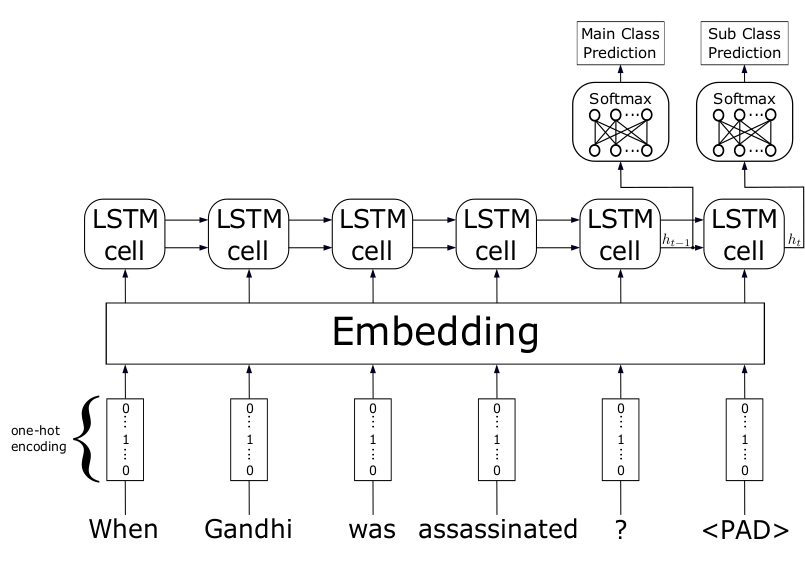
\includegraphics[scale=0.35]{../images/lstm-intent2.png}
			\caption{Basic classification model using RNNs \citep{lstmintent}}\label{lstmIntent2}
		\end{figure}
		To verify their results \citep{lstmintent} implemented a prototype responder by adding a biLSTM on top of the LSTM layer seen in figs. \ref{lstmIntent1} and \ref{lstmIntent2}.  The biLSTM model uses the predictions from the previous layer, both main and subclass predictions, and combines them to form the final output.

		\subsection{Critical Issues in LSTMs}\label{c2criticalissues}

		From the literature reviewed so far, it has become apparent that LSTMs generate a view of the world in a very sequential manner. While successful in managing banishing gradients and generating better, contextually relevant results, LSTMs or even biLSTMs aren't entirely correct, with none of the models achieving over 90\% accuracy across various datasets consistently. LSTMs suffer from another fatal flaw, their sequential nature makes it extremely difficult to parallelize the work and this leads to extended training times, out of memory errors etc.

	    \section{Transformers}\label{23}

	    	The previous section highlighted some key advancements in the field of machine comprehension and LSTMs, however, not a lot changed for almost two decades in the field of NLP based machine comprehension tasks architecturally. Since their introduction in 1997, LSTMs \citep{lstmoriginal} have been the base architecture for countless applications. However, as we noted in section \ref{c2criticalissues}, LSTMs have some critical drawbacks.

			\textit{Transformers} were introduced in late 2017 by \citep{atayl} and have become a very reliable way to implement various NLP based tasks. The basic architecture for which can be seen in fig. \ref{transformerArchitecture}.
			\begin{figure}[h!]
				\centering
				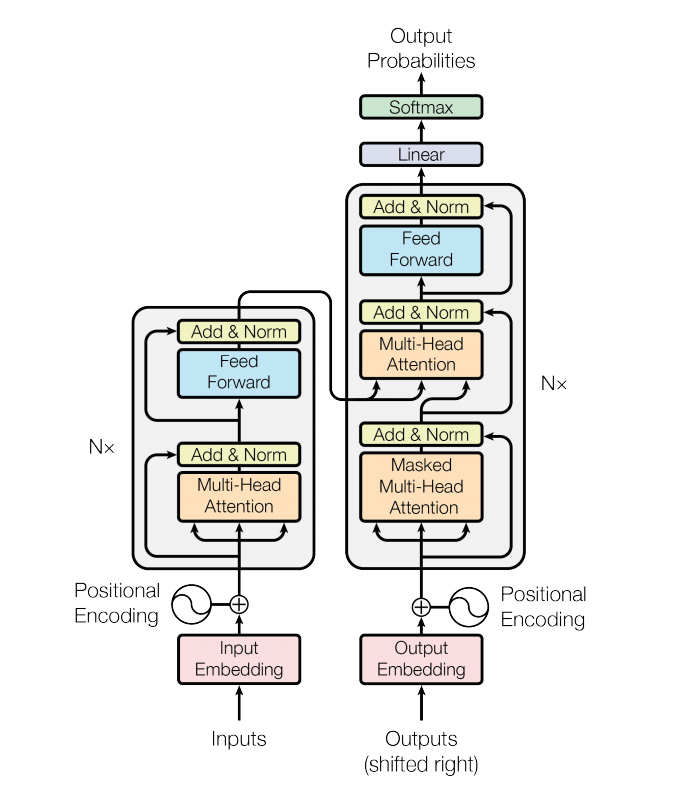
\includegraphics[scale=0.4]{../images/transformer.png}
				\caption{Transformer Architecture built by \citep{atayl}}\label{transformerArchitecture}
			\end{figure}
	        Recurrent models usually adopt a combination approach where they take symbol position of the input and output positions along with the computation. This helps them align positions to steps in computation time and generate a sequence of hidden states $ h_{t} $, which is a function of the previous hidden state $ h_{t-1}$ and the input function $ t $.  This inherently sequential nature of RNNs causes memory issues, leading to reduced batch sizes.

			The architecture for a \textit{Transformer} in this paper is outlined as having an encoder that maps input sequences to a continuous representation. The architecture can be seen in Fig. \ref{transformerArchitecture}. This is then decoded into an output sequence of symbols one at a time. Each step is auto-regressive, ie. it consumes the previously generated symbols as additional input when creating the next. This is similar to an ensemble model. Stacks of 6 encoder and 6 decoder layers is used.\\
			Each encoder layer has 2 sub-layers of a multi-head self-attention and the other a simple, position-wise fully connected feed-forward network layer. The output from each encoder layer can be represented as $  LayerNorm(x + Sublayer(x)) $, where $ Sublayer(x) $ is the function implemented by the sub-layers in the model. Additionally, supporting residual connections is handled by producing outputs of dimension $ d_{model}=512 $.

			The decoder layer is similar to the encoder layer and has an additional 3rd sub-layer that performs multi-head attention over the output of the encoders. To ensure that the output layer isn't affected by the output of residual connections from the sub-layers, a normalization layer is implemented at the end. Masking the subsequent positions and offsetting the output by 1 position ensures that the predictions for position $ i $ can only depend on outputs from previous positions.

            The \textit{Transformer} architecture was the first one to implement a self-attention based transduction model to compute input and output representations without the use of convolution or sequence-aligned networks.

			One of the key features in a Transformer architectures is \textit{self-attention}, which is covered in-depth in section \ref{231}.

			\subsection{Self Attention}\label{231}

            In their paper ``Attention Is All You Need", \citep{atayl} highlight that \textit{self-attention} is a key piece of the puzzle. This is due to several reasons such as the ability to parallelize computation, reduce total complexity per layer and the reduced path lengths between various long-range dependencies in the network. It is easier to learn about these dependencies if the distance between them is shorter.
            Thus, the transformer also computes the length of the longest path between any two input-output positions.

            The attention mechanism was designed by \citep{attentioneMech} to solve a critical issue with encoder-decoder architecture dependent LSTM and RNN based models. As has been highlighted before, LSTMs suffer from an inability to retain long-range sequence dependencies. Using a (soft)-search approach allows the model to look for parts that are relevant to predicting an output sequence, rather than forming all the segments of a sentence produces better results than existing fixed-length encoder-decoder models.
            The (soft)-search is performed after a prediction is made. This prediction is based on a set of positions for the source sentence, where the target word has the highest concentration of context vectors associated with previously generated target words. Another distinguishing feature of the attention mechanism is that it does not try to encode an entire input sentence to a fixed-length vector. Rather, it encodes the input sentence into sequence vectors that can be adaptively decoded during translation. Thus freeing the model from having to squash a lot of information from the source sentence into a vector of fixed-length.

			The work done in \citep{atayl} modified that attention mechanism by mapping a query to a set of key-value pairs and developing \textit{self-attention}. To understand self attention take an example sentence like:
            \\\\
            \textit{``The lion was resting in the shade because it was tired after hunting."}\\

             While this is a perfectly normal sentence to a human being, a computer does not know what ``it" means and that ``it" refers to the ``lion" in the second half of this sentence. Self- attention allows a Transformer to understand that the word ``it" refers to the ``lion" in this context.
             In fig. \ref{multiHeadAttention} shows how \citep{atayl} modified the attention mechanism.
			\begin{figure}[h!]
				\centering
				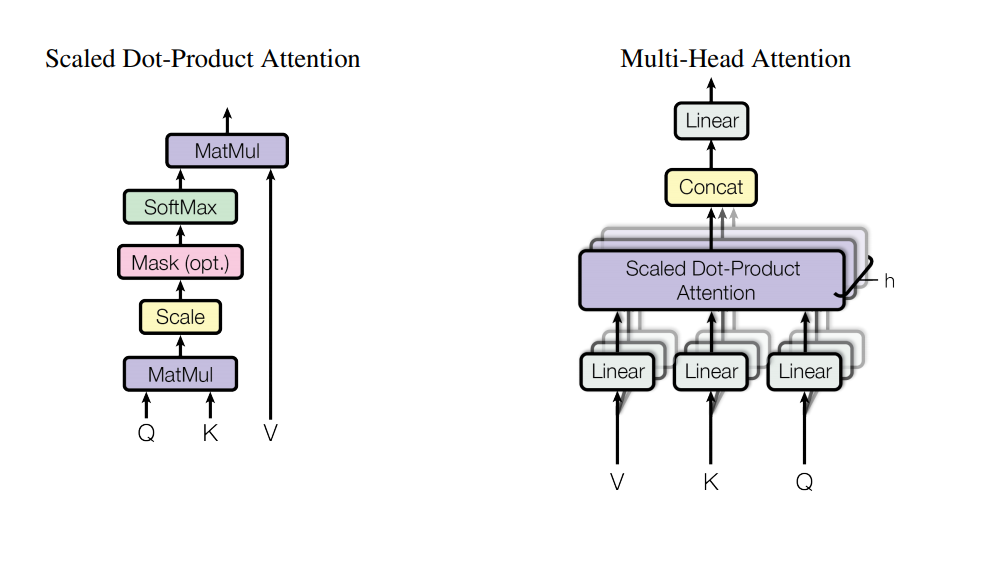
\includegraphics[scale=0.4]{../images/multihead.png}
				\caption{Scale Dot and Multi-Head Attention Models \citep{atayl}}\label{multiHeadAttention}
			\end{figure}

            The ``Scaled Dot-Product Attention" layer implemented in the transformer works by computing the dot products of all the input query with all the keys, divide it by the dimension of the keys and finally apply a softmax function to obtain the weights. This can be represented as:

            \begin{equation}\label{attentionEq}
                Attention(Q,K,V)=softmax\bigg(\dfrac{QK^{T}}{\sqrt{d_k}}\bigg)V
            \end{equation}
            where $ K, V $ are the matrices containing the keys and values respectively, and $ Q $ is the set of queries. The dimension of the keys is given by $ d_k $. The dot product is used because it is more efficient than the additive attention product and is faster as well \citep{atayl}.

            Instead of using single attention, the transformer implements \textit{multi-head} attention.  Multi-head attention, which can be seen in fig. \ref{multiHeadAttention} on the right, allows for the model to simultaneously gather information from various different representations in different subspaces and positions.
            \begin{equation}\label{multiheadEQ}
            \begin{aligned}
               \text{MultiHead}(Q,K,V) = Concat(head_1,...,head_h)W^O \\
                \text{where head}_{\mathrm{i}}=\text { Attention }\left(Q W_{i}^{Q}, K W_{i}^{K}, V W_{i}^{V}\right)
            \end{aligned}
           \end{equation}

            Matrices $W_{i}^{Q} \in \mathbb{R}^{d_{\text {model }} \times d_{k}}, W_{i}^{K} \in \mathbb{R}^{d_{\text {model }} \times d_{k}}, W_{i}^{V} \in \mathbb{R}^{d_{\text {mod } 1} \times d_{v}}$ and $W^{O} \in \mathbb{R}^{h d_{v} \times d_{\text {model }}}$ represent the projection parameters. They also implemented $h=8$ parallel attention/head layers. The reduced dimensionality of each head with $d_{k}=d_{v}=d_{\text {model }} / h=64$ means that the total cost is similar to a fully connected, single-head attention layer.
            The evaluations performed on the Wall Street Journal dataset\citep{wsj}, using 40k sentences, showed that even without task-specific tuning the model had better results with a fraction of the training cost.

            The advantages of the Transformer architecture are clearly evident over the standard RNN based LSTMs and other architectures. Experiments on the WMT 2014 English to German translation \citep{wmt} using the big transformer showed a significant jump in BLEU score 28.4 over various other seq2seq models and even combined ensemble models which earlier had a highest score of 26.36 using a ConvS2S Ensemble \citep{convs2s}.


		\subsection{Improvements of Transformer Architectures}\label{232}

            Transformers have significant advantages as highlighted earlier. Improvements to the basic architecture are discussed below.
		\subsubsection{BERT}\label{2321}

			The paper on \textit{Bidirectional Encoder Representations from Transformers} (BERT) \citep{bert}, introduces a new language model. This model is truly fascinating in many ways. First and foremost it is designed to pre-train deep bidirectional representations using unlabelled data. This is done by jointly conditioning context in all layers to the right and left. This pre-training allows the model to be fine-tuned simply using one additional output layer. These features make this model conceptually simple and very powerful empirically.

			BERT employs language pre-training \citep{dai, deepContextualized, radford2018improving} which has shown significant advantages in many applications e.g. paraphrasing, language level inference etc. These tasks aim to highlight the relationships between sentences through contextual understanding as well as by using tokenized outputs. BERT improves on the fine-tuning tasks that are important to performing
			\begin{figure}[h!]
				\centering
				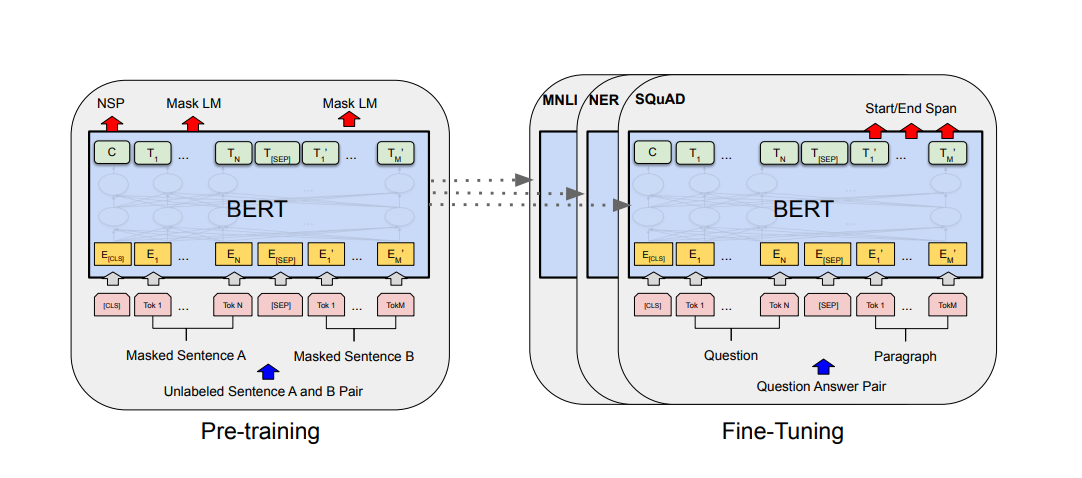
\includegraphics[scale=0.35]{../images/BERT.png}
				\caption{Pre-training and Fine Tuning procedures for BERT \citep{bert}}\label{bertPretraining}
			\end{figure}

			BERT was tested on The General Language Understanding Evaluation (GLUE) benchmark \citep{wang} which has a large number of diverse NLU tasks.
			BERT performed extremely well on the 11 NLP tasks that the authors ran it against. It showed an average accuracy improvement of 4.5\% and 7\% when compared to the previous state of the art models. Results of BERT and its significant gains make it one of the best candidate models for NLU tasks.

	       \subsubsection{ALBERT}\label{2322}
	       \citep{albert}

	       \subsubsection{ROBERTA}\label{2323}
	       \citep{roberta}

	       \subsubsection{DISTILBERT}\label{2324}
	       \citep{distil}

        \section{Summary}\label{26}


    \chapter{Research Methodology}\label{c3researchmeth}
    
    Before diving into anything, lets take a look at a rough flow diagram:
    \newpage
    \resizebox{\columnwidth}{!}{

		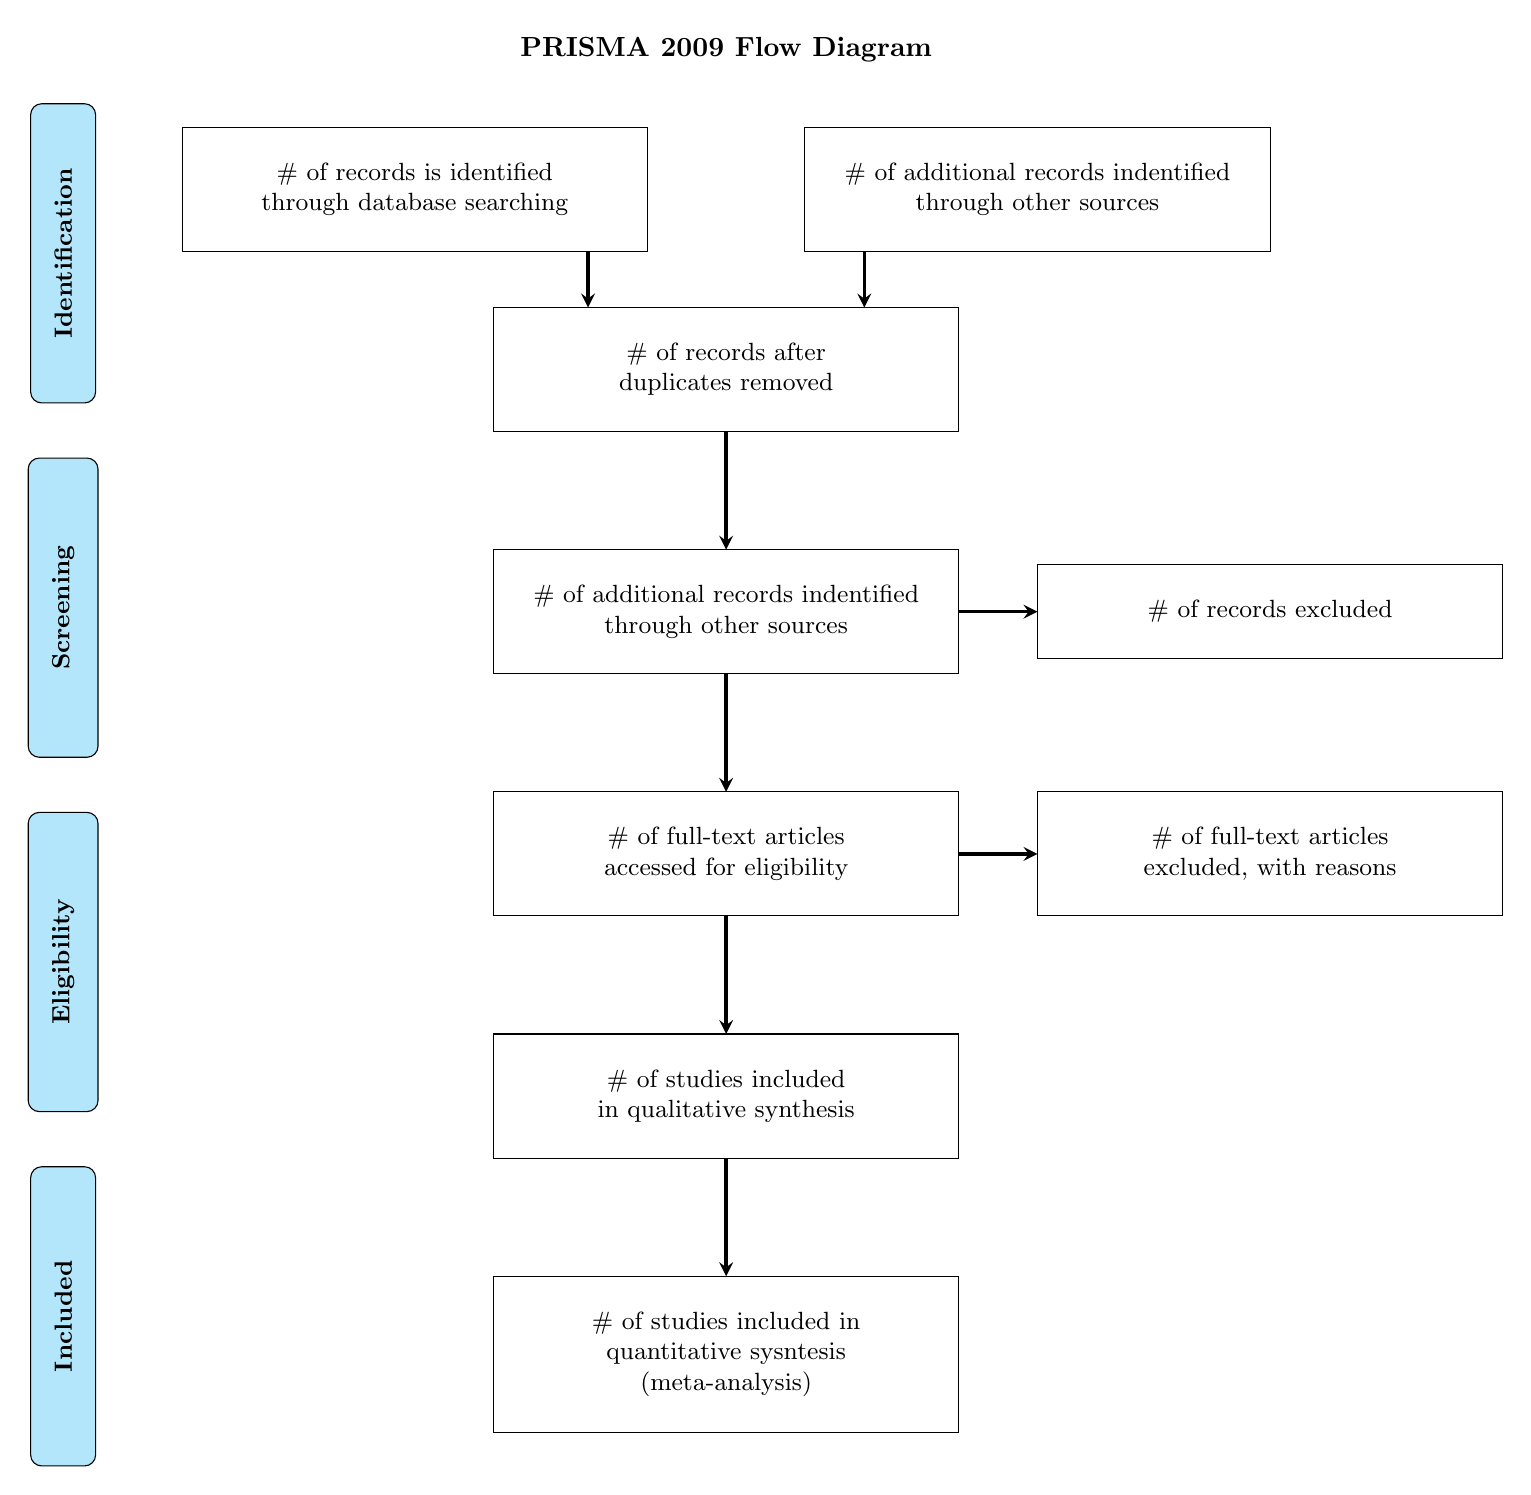
\begin{tikzpicture}[
		node distance=15mm and 10mm,
		start chain=going below,
		mynode/.style = {
			draw, rectangle, align=center, text width=5cm,
			font=\small, inner sep=3ex, outer sep=0pt,
			on chain},
		mylabel/.style = {
			draw, rectangle, align=center, rounded corners, 
			font=\small\bfseries, inner sep=2ex, outer sep=0pt,
			fill=cyan!30, minimum height=38mm,
			on chain},
		every join/.style = arrow,
		arrow/.style = {very thick,-stealth}
		] 
		\coordinate (tc);
		% the title
		\node[above=of tc,font=\bfseries] {PRISMA 2009 Flow Diagram};
		% the nodes at the top
		\node (n1a) [mynode, left=of tc]    {\# of records is identified 
			through database searching};
		\node (n1b) [mynode,right=of tc]    {\# of additional records indentified\\
			through other sources};
		% the chain in the center
		\node (n2)  [mynode, below=of tc]   {\# of records after duplicates removed};
		\node (n3)  [mynode,join]   {\# of additional records indentified\\
			through other sources};
		\node (n4)  [mynode,join]   {\# of full-text articles accessed 
			for eligibility};
		\node (n5)  [mynode,join]   {\# of studies included in qualitative synthesis};
		\node (n6)  [mynode,join]   {\# of studies included in quantitative sysntesis\\
			(meta-analysis)};
		% the branches to the right
		\node (n3r) [mynode,right=of n3]    {\# of records excluded};
		\node (n4r) [mynode,right=of n4]    {\# of full-text articles excluded,
			with reasons};
		% lines not included in join                                        
		\draw[arrow] ([xshift=+22mm] n1a.south) coordinate (a)
		-- (a |- n2.north);
		\draw[arrow] ([xshift=-22mm] n1b.south) coordinate (b)
		-- (b |- n2.north);
		\draw[arrow] (n3) -- (n3r);
		\draw[arrow] (n4) -- (n4r);
		% the labels on the left
		\begin{scope}[node distance=7mm]
			\node[mylabel,below left=-3mm and 11mm of n1a.north west]
			{\rotatebox{90}{Identification}};
			\node[mylabel]  {\rotatebox{90}{Screening}};
			\node[mylabel]  {\rotatebox{90}{Eligibility}};
			\node[mylabel]  {\rotatebox{90}{Included}};
		\end{scope}
	\end{tikzpicture}
}

    \section{Data Selection}\label{c31}

    	We have selected the Stanford Question Answering Dataset (SQuAD). This is as a reading comprehension dataset based on Wikipedia articles. It is based on questions posed by crowd-workers on a set of articles. The answer to every question is a segment of text or span, from the corresponding reading passage, or the question might be unanswerable \citep{dataset}.

    	The dataset consists of over 150,000 questions. Split into 100,000 answerable and 50,000+ unanswerable question, which were written to look similar to unanswerable questions. The challenge being that a model should be able to correctly answer the answerable questions and abstain from answering the unanswerable ones.
	    The dataset is freely available as a part of the Transformers package in python or it can be downloaded from the SQuAD 2.0 website \citep{squad}.

	    To effectively use this dataset for our purposes, let us first take a look at what its contents look like below.\\ \\
	    \noindent\fbox{
	    	\parbox{\textwidth}{\textbf{Context:}\textit{``The Normans (Norman: Nourmands; French: Normands; Latin: Normanni) were the people who in the 10th and 11th centuries gave their name to Normandy, a region in France. They were descended from Norse ("Norman" comes from "Norseman") raiders and pirates from Denmark, Iceland and Norway who, under their leader Rollo, agreed to swear fealty to King Charles III of West Francia."}\\
	    		\textbf{Question: } \textit{Who was the Norse leader?}\\
	    		\textbf{Answer: } \textit{Rollo}}
	    }
	    \newline
	    \newline

	    The answer to the aforementioned question is quite simple for humans to comprehend. The challenge is for us to contextualize this and make it machine-understandable so that our model can answer it correctly.

	    The dataset consists of various kinds of English language examples like negation, antonyms, entity swaps, impossible conditions to answer, answerable, etc. making the dataset a well-balanced one.

	    To use this dataset correctly we shall perform the following pre-processing steps on it:

	    \begin{enumerate}
	    	\item Data splitting into separate Question, Answer and Context lists.
	    	\item Splitting the data into separate training and validation sets of  question and answers using the 80/20 rule, also known as the Pareto principle. We will have 80\% training data and 20\% test data.
	    	\item Tokenization of the split data to generate "context-question" pairs
	    	\item Generating indexes for when an answer begins and ends in the dataset
	    	\item Adding answer tokens based on their encoded positions
	    \end{enumerate}

        The SQuAD 2.0 Dataset \citep{dataset}, was developed with funding from Facebook to help address some major issues with existing datasets. Most datasets focus on questions that can be easily answered or use of    automatically generated, unanswerable questions which are easily identifiable.\\
        The SQuAD 2.0 dataset resolves this by combining the SQuAD dataset along with 50,000 crowd worker generated unanswerable questions. The key feature of these being that the unanswerable questions must look similar to answerable ones. For a model to be successful on this new dataset, it must be able to answer all possibly answerable questions as well as determine when no answers are provided for a question in the given paragraph and abstain from answering. A comparative study was done for a Natural Language Understanding(NLU) task that obtained an 86\% score on SQuAD 1.1, only got 66\% on the new 2.0 dataset.
        The dataset helps bridge the gap between true NLU and machine understanding by using the concept of Relevance. Through comparisons with various datasets such as RACE, MCTest, QASENT etc. they have identified the missing links like negative examples, antonyms and helped fill the gap. This dataset forces the models to understand whether a paragraph span has the answer to the question posed.

		\begin{table}[h!]
		              \centering
		                \begin{tabular}{|l|l|l|}
		                    \hline
		                     & SQuAD 1.1 &  SQuAD 2.0 \\
		                    \hline
		                    \textbf{Train} & & \\
		                        Total Examples & 87,599 &  130,319 \\
		                        Negative Examples & 0 & 43,498 \\
		                        Total articles & 442 & 442 \\
		                        Articles with negatives & 0 & 285 \\
		                    \hline
		                    \textbf{Development} & & \\
		                        Total Examples & 10,570 &  11,873 \\
		                        Negative Examples & 0 & 5,945 \\
		                        Total articles & 48 & 35 \\
		                        Articles with negatives & 0 & 35 \\
		                    \hline
		                    \textbf{Test} &  & \\
		                        Total Examples & 9,533 & 8,862 \\
		                        Negative Examples & 0 & 4,332 \\
		                        Total articles & 46 & 28 \\
		                        Articles with negatives & 0 & 28 \\
		                    \hline
		                \end{tabular}
		                \caption{Comparison of  SQuAD 2.0 to SQuAD 1.1\citep{dataset}.}\label{datasetDescription}
		 \end{table}

    Table \ref{datasetDescription} shows the difference between
    \section{Data Pre-processing And Transformation}\label{c32}
    Techniques used.
    (1) Average pooling; (2) max pooling; (3) the concatenation of the last vectors on both directions. Dropout operation is performed on the QA representations before cosine similarity matching. Use GloVe embeddings and suffix-prefix encoding in both directions of self attention pass to show improvements.
    \section{Research Hypothesis}\label{c33}
    The hypothesis of this research is that implementing a self attention based Transformer model with:
    \begin{itemize}
    	\item glove embedding
    	\item BERT base\citep{bert}
    	\item Answer pointer output layer\citep{lstmPointer, lstmhu2016question}

    \end{itemize}
	\section{Model Evaluation Metrics}\label{33}
	
		To successfully evaluate the model two metrics will be used. The \textit{F1 - Score} and \textit{Exact Match Score} will be used to measure the success of the model developed. While accuracy is a good score to measure how well a model is performing, the problem with accuracy is that it is prone to overfitting, and underfitting, which might lead to great accuracy scores but real world predictions wont be as accurate.
		
		Accuracy also doesn't work because it is a simplistic probability metric that assumes both false positives and false negatives have an equal weight in predicting the outcome as shown in eq. \ref{accuracy}.
				\begin{equation}\label{accuracy}
			Accuracy = \dfrac{True Positive +  True Negative}{True Positive +  False Positive + True Negative +  False Negative}
		\end{equation}
	\\
		Outlined below are some reasons why accuracy is not a good measure:
		\begin{enumerate}
			\item \textbf{Class Imbalance}
			\item \textbf{Prone to Over and Underfitting}
		\end{enumerate}

	Precision
	
	Recall
	
	F1 Score 
	
	Exact Match
	
  \chapter{Architecture Creation}\label{c4}

     In this cahpter we yaba daba do
       \section{Drawbacks Of Current Architectures}\label{c42}
       \section{Proposed Architecture Improvements}\label{c43}
       \section{Architecture Refinement}\label{c44}
       
    \chapter{Results And Discussion}\label{c5}
     \section{Existing Models And Benchmarks}\label{c41}
    
    To be able to establish the improvements hypothesized in the previous section it is important to have a baseline metric. The BERT \citep{bert}, ALBERT \citep{albert}, RoBERTa \citep{roberta} and DistilBERT \citep{distil} models are available pre-trained through the HuggingFace library \citep{hfTransformers}. The library also provides the SQuAD 2.0 Dataset \citep{dataset} for use.
    
    Each of these models will be run for 10 epochs, their training loss, EM and F1 scores will be taken as baseline metrics against which the improved model will be compared.
    \begin{figure*}
    	\centering
    	\begin{subfigure}[b]{0.475\textwidth}
    		\centering
    		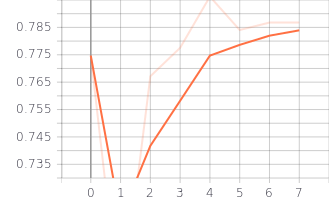
\includegraphics[width=\textwidth]{../images/Albert_Val_F1.png}
    		\caption{{\small AlBert Validation F1 Score}}    
    		\label{fig:mean and std of net14}
    	\end{subfigure}
    	\hfill
    	\begin{subfigure}[b]{0.475\textwidth}  
    		\centering 
    		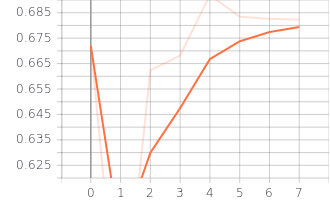
\includegraphics[width=\textwidth]{../images/Albert_Val_EM.png}
    		\caption{{\small AlBert Validation Exact Match}}    
    		\label{fig:mean and std of net24}
    	\end{subfigure}
    	\vskip\baselineskip
    	\begin{subfigure}[b]{0.475\textwidth}   
    		\centering 
    		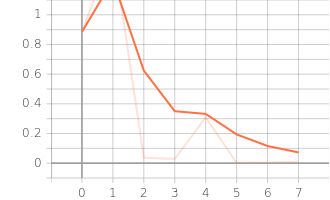
\includegraphics[width=\textwidth]{../images/Albert_Val_Loss.png}
    		\caption{{\small AlBert Validation Loss}}    
    		\label{fig:mean and std of net34}
    	\end{subfigure}
    	\hfill
    	\begin{subfigure}[b]{0.475\textwidth}   
    		\centering 
    		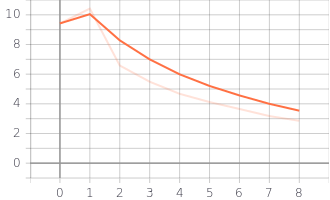
\includegraphics[width=\textwidth]{{../images/Albert_Train_Loss.png}}
    		\caption
    		{{\small AlBert Training Loss}}    
    		\label{fig:mean and std of net44}
    	\end{subfigure}
    	\caption{ AlBert Model Benchmarks} 
    	\label{albertBenchmarks}
    \end{figure*}
    \chapter{Conclusions And Recommendations}\label{c6}
    
    Through this work the author has attempted to highlight the advancements and propose a unique modification to the existing transformer architecture using an Answer-Pointer network. 
    
    \section{Recommendations}
    
    This work provides a unique opportunity to introduce improvements to an already state of the art architecture by adding a layer of LSTM based pointers. Highlighted below are some recommendations, that the author believes, can improve the architecture further.
    
    \begin{itemize}
    	
    	\item \textbf{Increased Batch-Size}: The experiments presented in this work are limited by a relatively small batch size of 8. Systemic increase of batch size can allow for reduced training times, possibly better performance overall and an opportunity to test this model against various other NLP applications such as Sequence Classification, Token Classification, Sentence Predictions, etc. 
    	\item \textbf{Better Hardware}: One of the key limiting factors for the work presented in this thesis is the limiting amount of VRAM, The current hardware used by the author only had 8GB of VRAM available on the EVGA 2070 Super GPU, which was insufficient for the benchmark batch size of 8. Reducing the batch size any further led to increased training times per epoch, upwards of 3 hours per epoch at a batch size of 6. This problem was slightly remediated by the use of Google Colab Pro, which is a subscriptions service that allows you to run experiments using better GPUs such as Tesla P100 GPU with 16GB VRAM. This service is time limited and thus not suitable for running long experiments. To effectively quantify the proposed architecture in this thesis it is recommended that it be run for at least 10 epochs on a multi-gpu setup that allows for mini-batches. This approach is discussed below.
    	\item \textbf{Mini-Batches Across Multiple GPUs}: Creating a multi-gpu setup, with 2 or more gpus, allows for accelerated training \citep{multigpu1}. A simple guide on how to set this up for PyTorch has been created on the Towards Data Science Medium page \citep{multigpu2} and even in the 
    \end{itemize}

   \setcitestyle{numbers}
    %\nocite{*}
    \bibliography{FinalThesis}
   \begin{appendices}
    	\chapter{Gantt Chart}\label{cgc}
		    \begin{figure}[!h]
		       	\centering
		        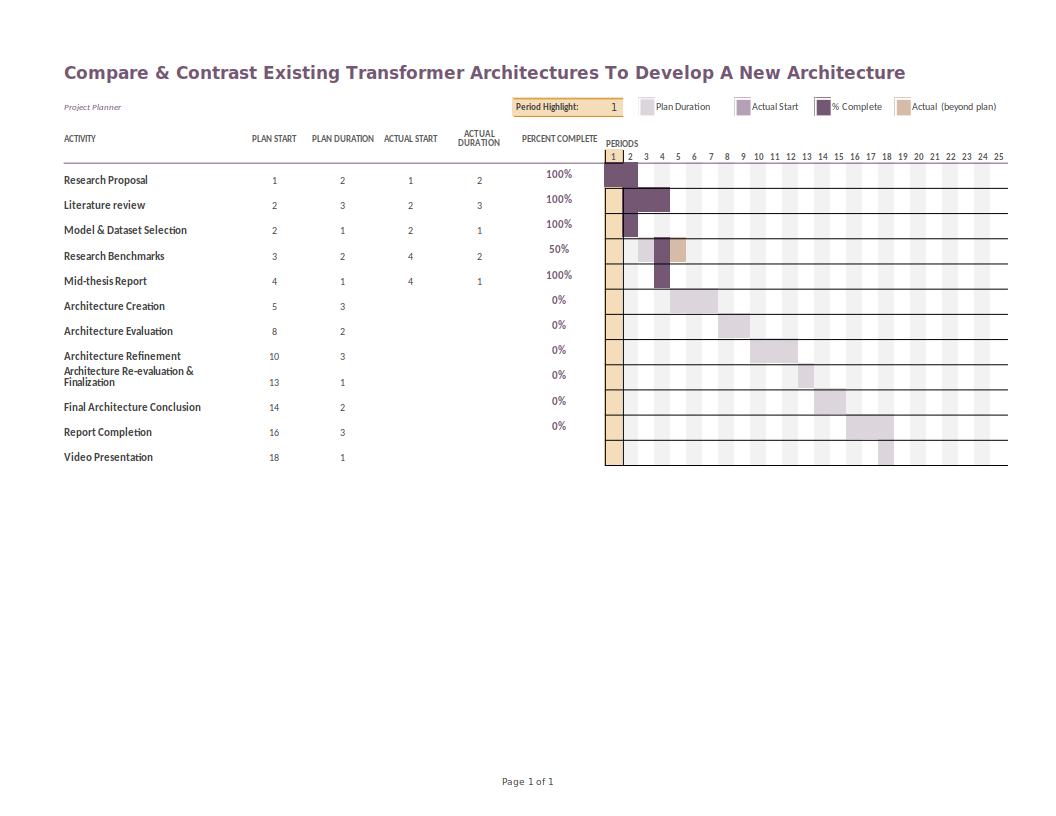
\includegraphics[scale=0.55,angle=90]{../images/GanttChart-mid.png}
		     	\caption{Mid-Thesis report Gantt Chart}\label{ganttChartMid}
              \end{figure}
         \chapter{Research Proposal}\label{crp}
         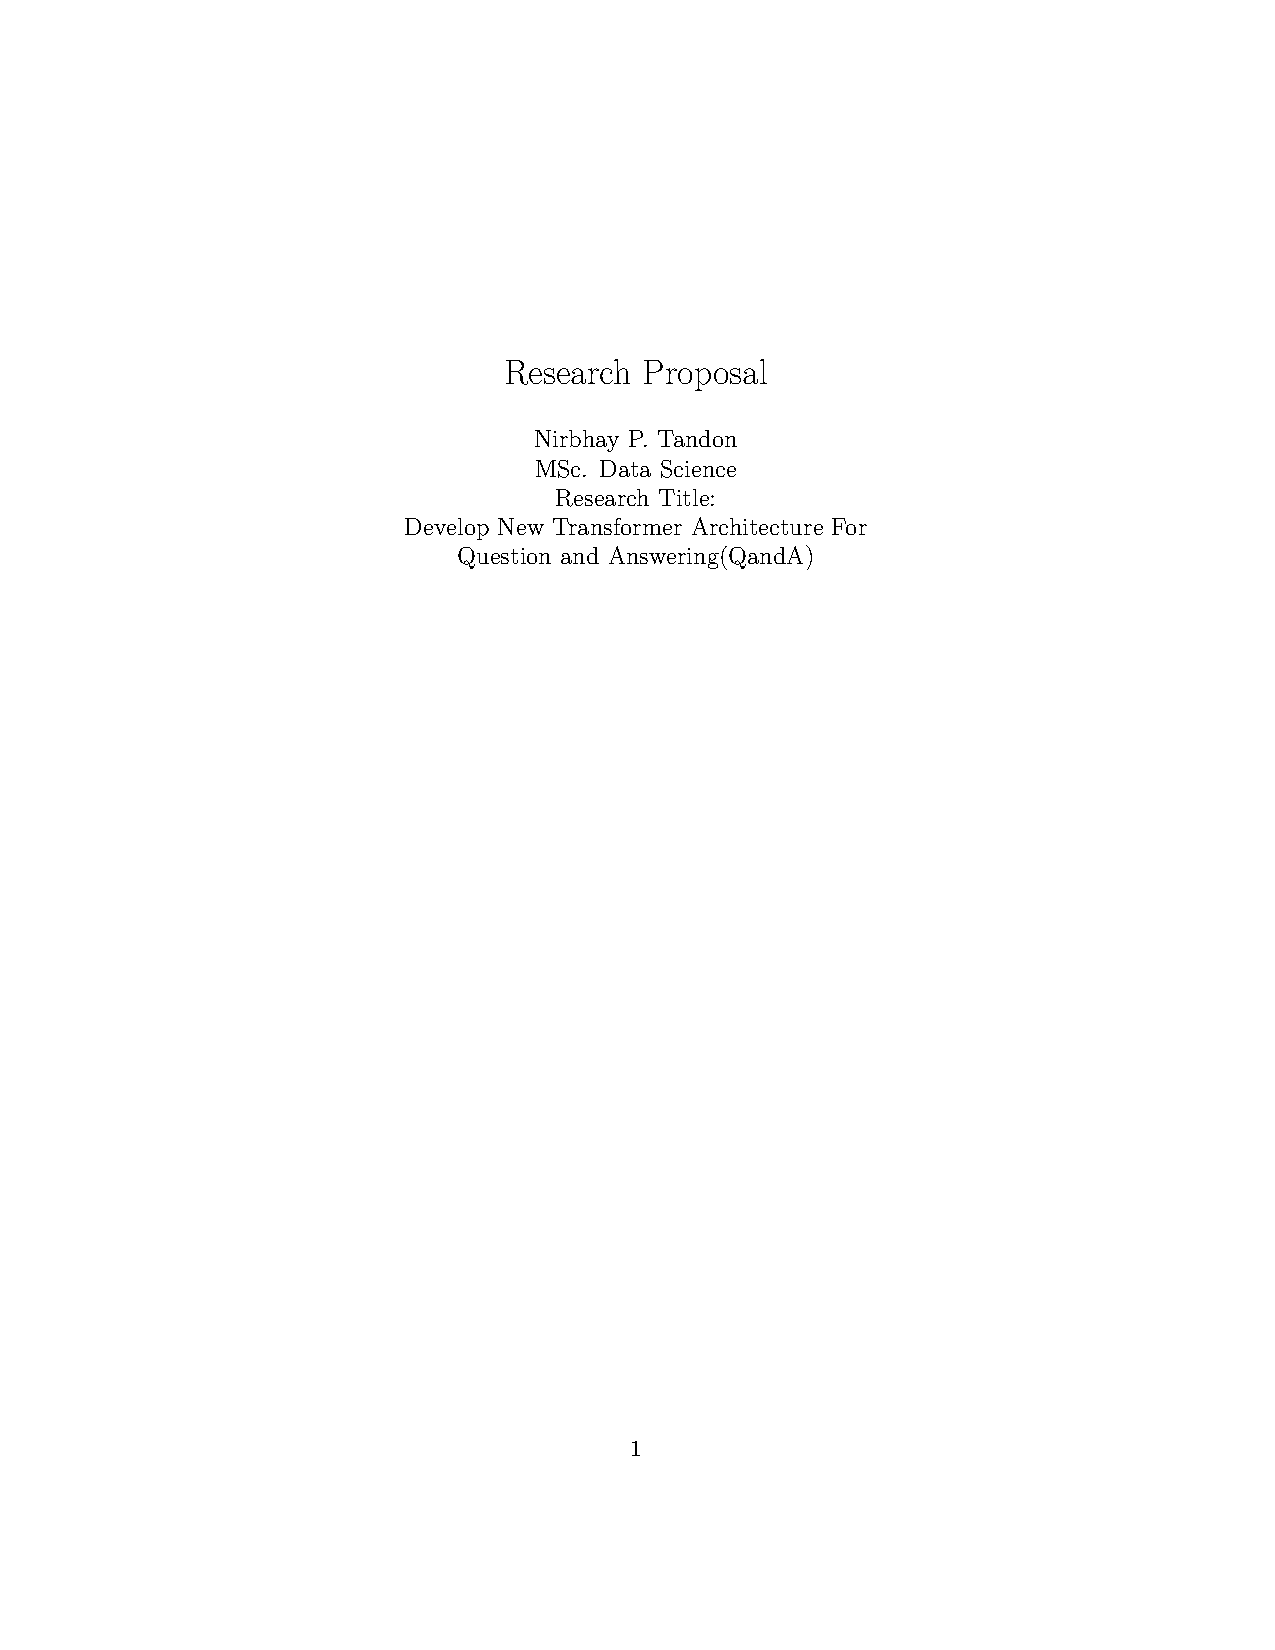
\includepdf[pages=1-15]{../rp.pdf}
    \end{appendices}


\end{document}